\chapter{Flight Testing and Performance Evaluation}\label{ch:performance}

\section{Simulation Results}
Simulation results were captured utilizing the \ac{APM} \ac{SITL} using X-Plane10.  The aircraft model chosen was an open-source flying wing model called the maxi-swift as seen in figure~\ref{fig:maxi-swift}.

\begin{figure}[!h]
 \centering
  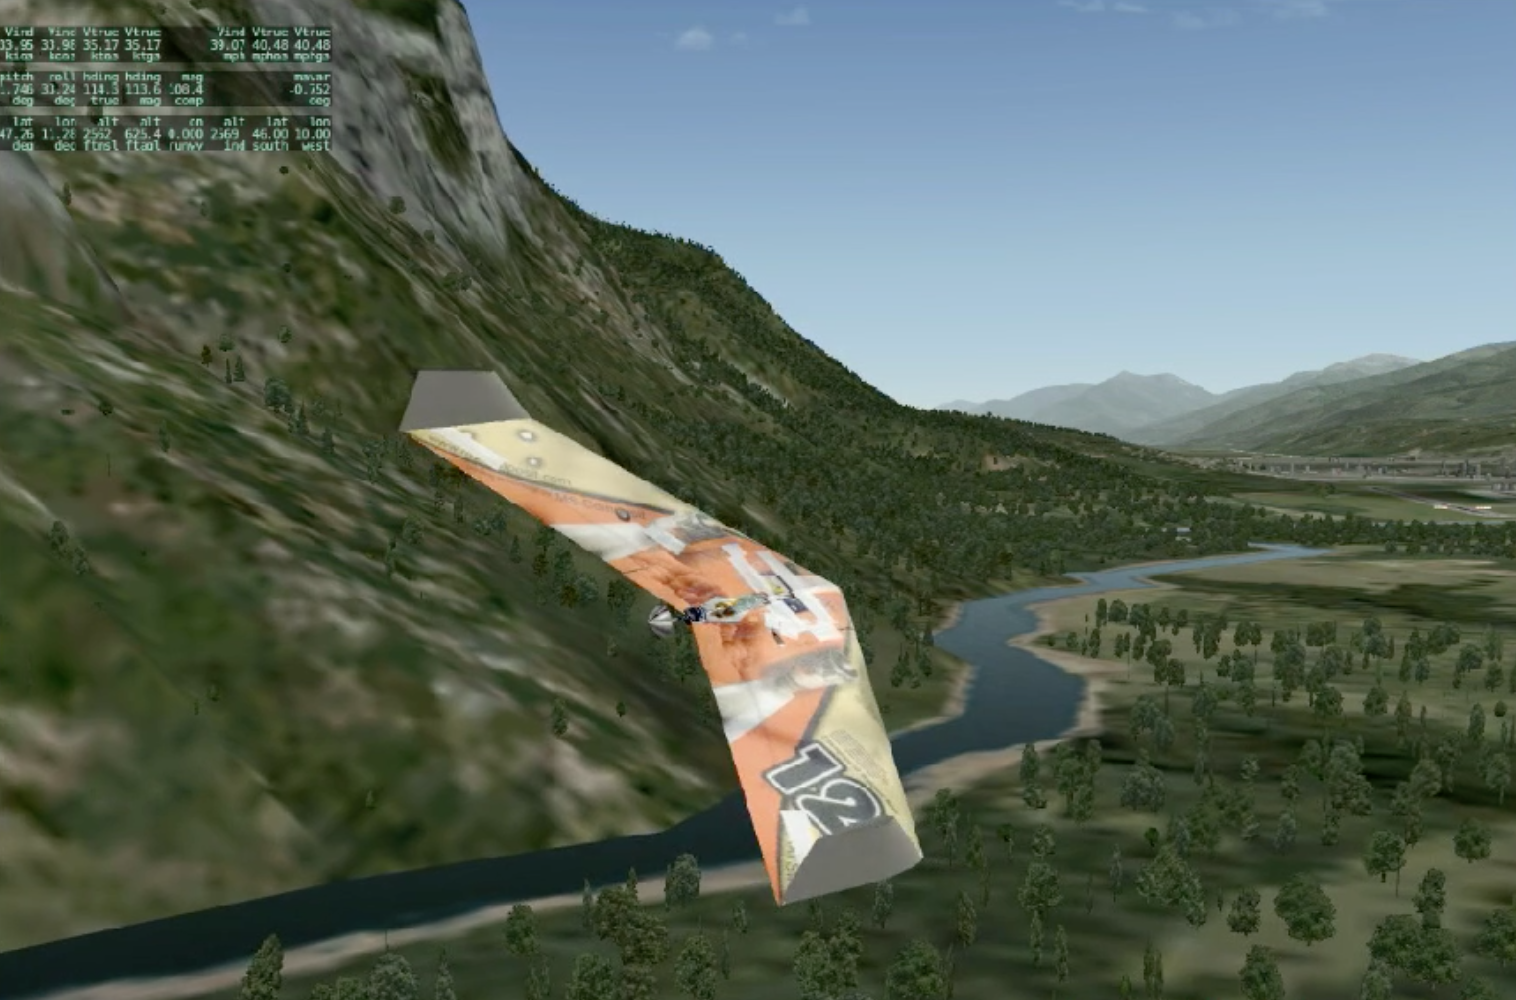
\includegraphics[width=0.75\textwidth]{maxi-swift.png}
  \caption{Maxi-Swift Flying Wing Model used in X-Plane10}
  \label{fig:maxi-swift}
\end{figure}
This plane did not afford proper testing of elevon mixing, but the fidelity in the model provided utilizing X-Plane10 was surprisingly accurate with respect to the FT-Spear aircraft used for actual flight test.  This drastically increased confidence that anything tested in \ac{SITL} would have a high probability of success in actual flight test.



\subsection{Pitch Attitude Performance}

It can be seen in figure~\ref{fig:pitch_perf} that there exists some steady state error when under \ac{PID} control.  This phenomenon is more pronounced when the desired pitch attitude is negative.  This steady state error is due to the increase in lift caused by the increasing airspeed.  The \ac{PID} controller underperforms in this regime.  However, the adaptive controller is able to compensate for these dynamics fast enough to track the desired attitude with no steady state error.

\begin{figure}[h!]
 \centering
  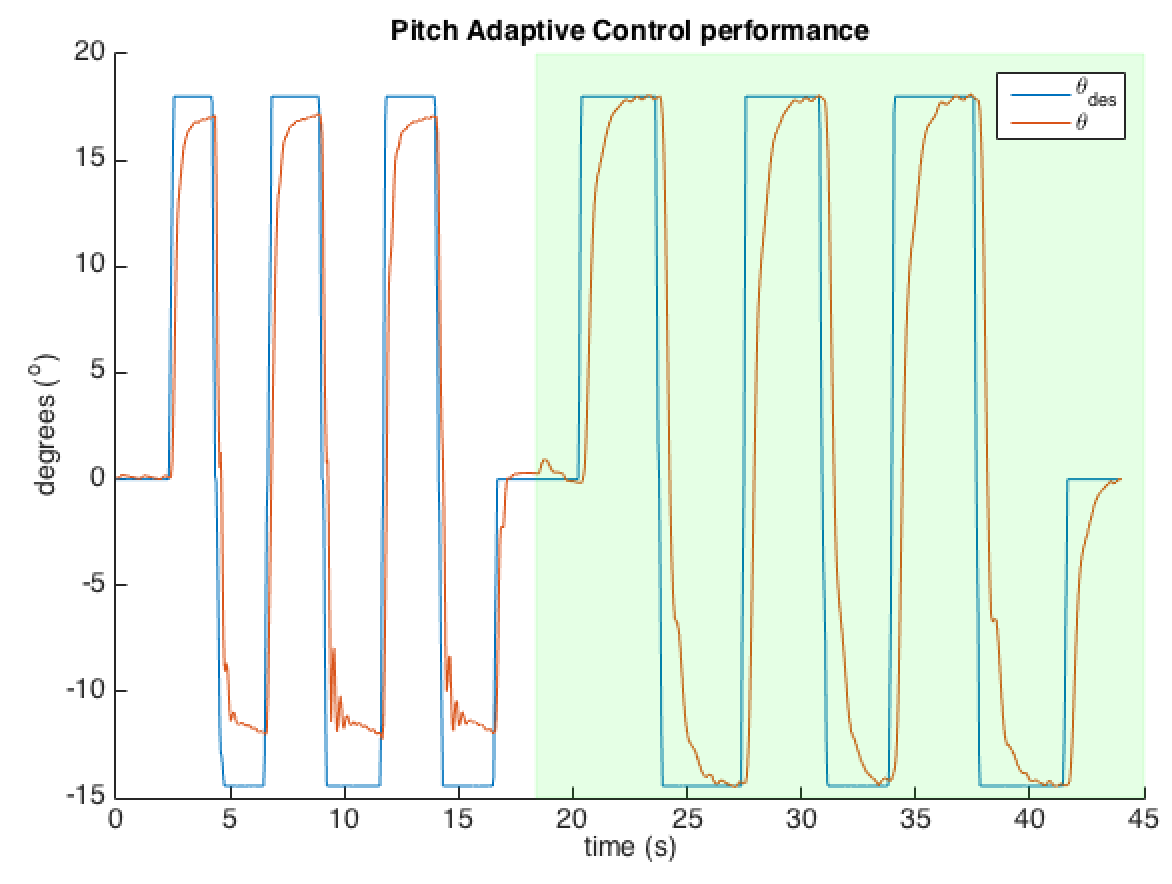
\includegraphics[width=1\textwidth]{pitch_perf.png}
  \caption{PID vs \Lone Adaptive Control Pitch Performance}
  \label{fig:pitch_perf}
\end{figure}

\subsection{Roll Induced Pitch Disturbance}
When rapidly rolling the maxi-swift aircraft in simulation, there was a noticeable coupling in the pitch axis.  The \ac{PID} controller struggles to correct this discrepancy because the time constant of the integral error simply cannot be increased high enough to achieve satisfactory compensation.  As seen in figure~\ref{fig:pitch_divergence}, the \Lone adaptive controller significantly reduced the pitching disturbance due to rapid rolling.

\begin{figure}[h!]
 \centering
  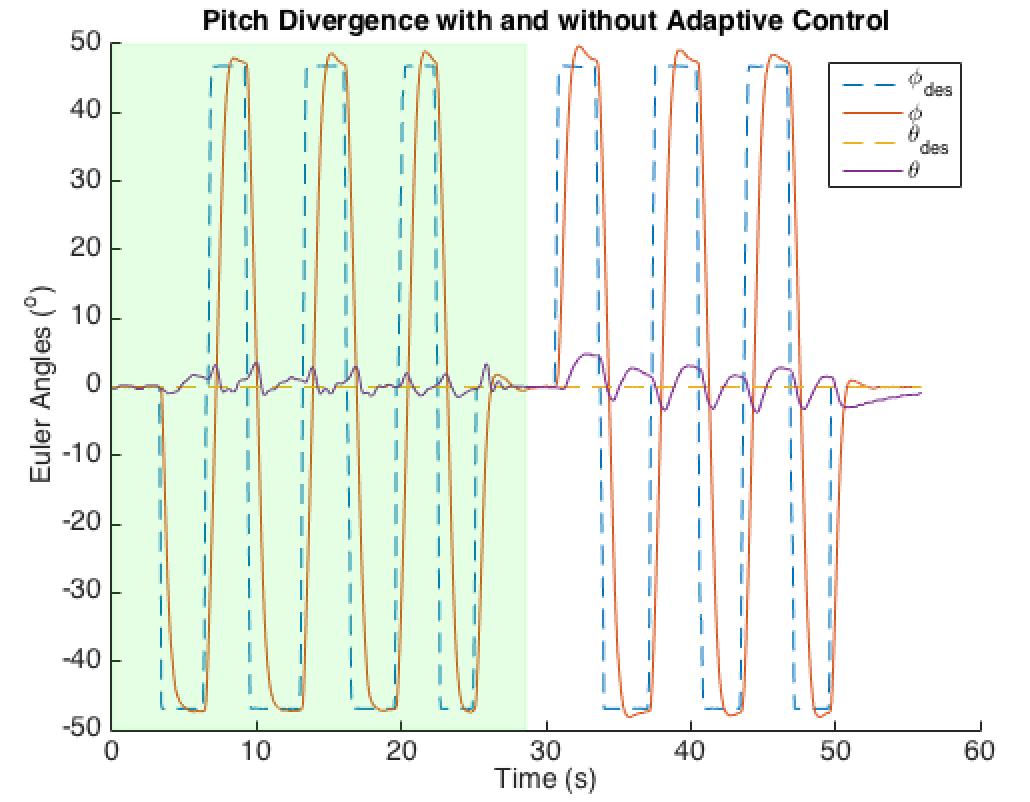
\includegraphics[width=1\textwidth]{pitch_divergence.png}
  \caption{PID vs \Lone Adaptive Control Coupled Pitch Resonse Performance}
  \label{fig:pitch_divergence}
\end{figure}

\subsection{Pitch due to Landing Gear and Flaps}
Lowering the landing gear and flaps entering the landing phase of flight causes un-commanded deviation in pitch.  The F4U Corsair (see figure~\ref{fig:corsair})in X-Plane10 was used to evaluate the attitude hold retention performance.  This un-modeled aerodynamics can cause the integrator in a \ac{PID} controller to saturate or wind up. 

\begin{figure}[h!]
 \centering
  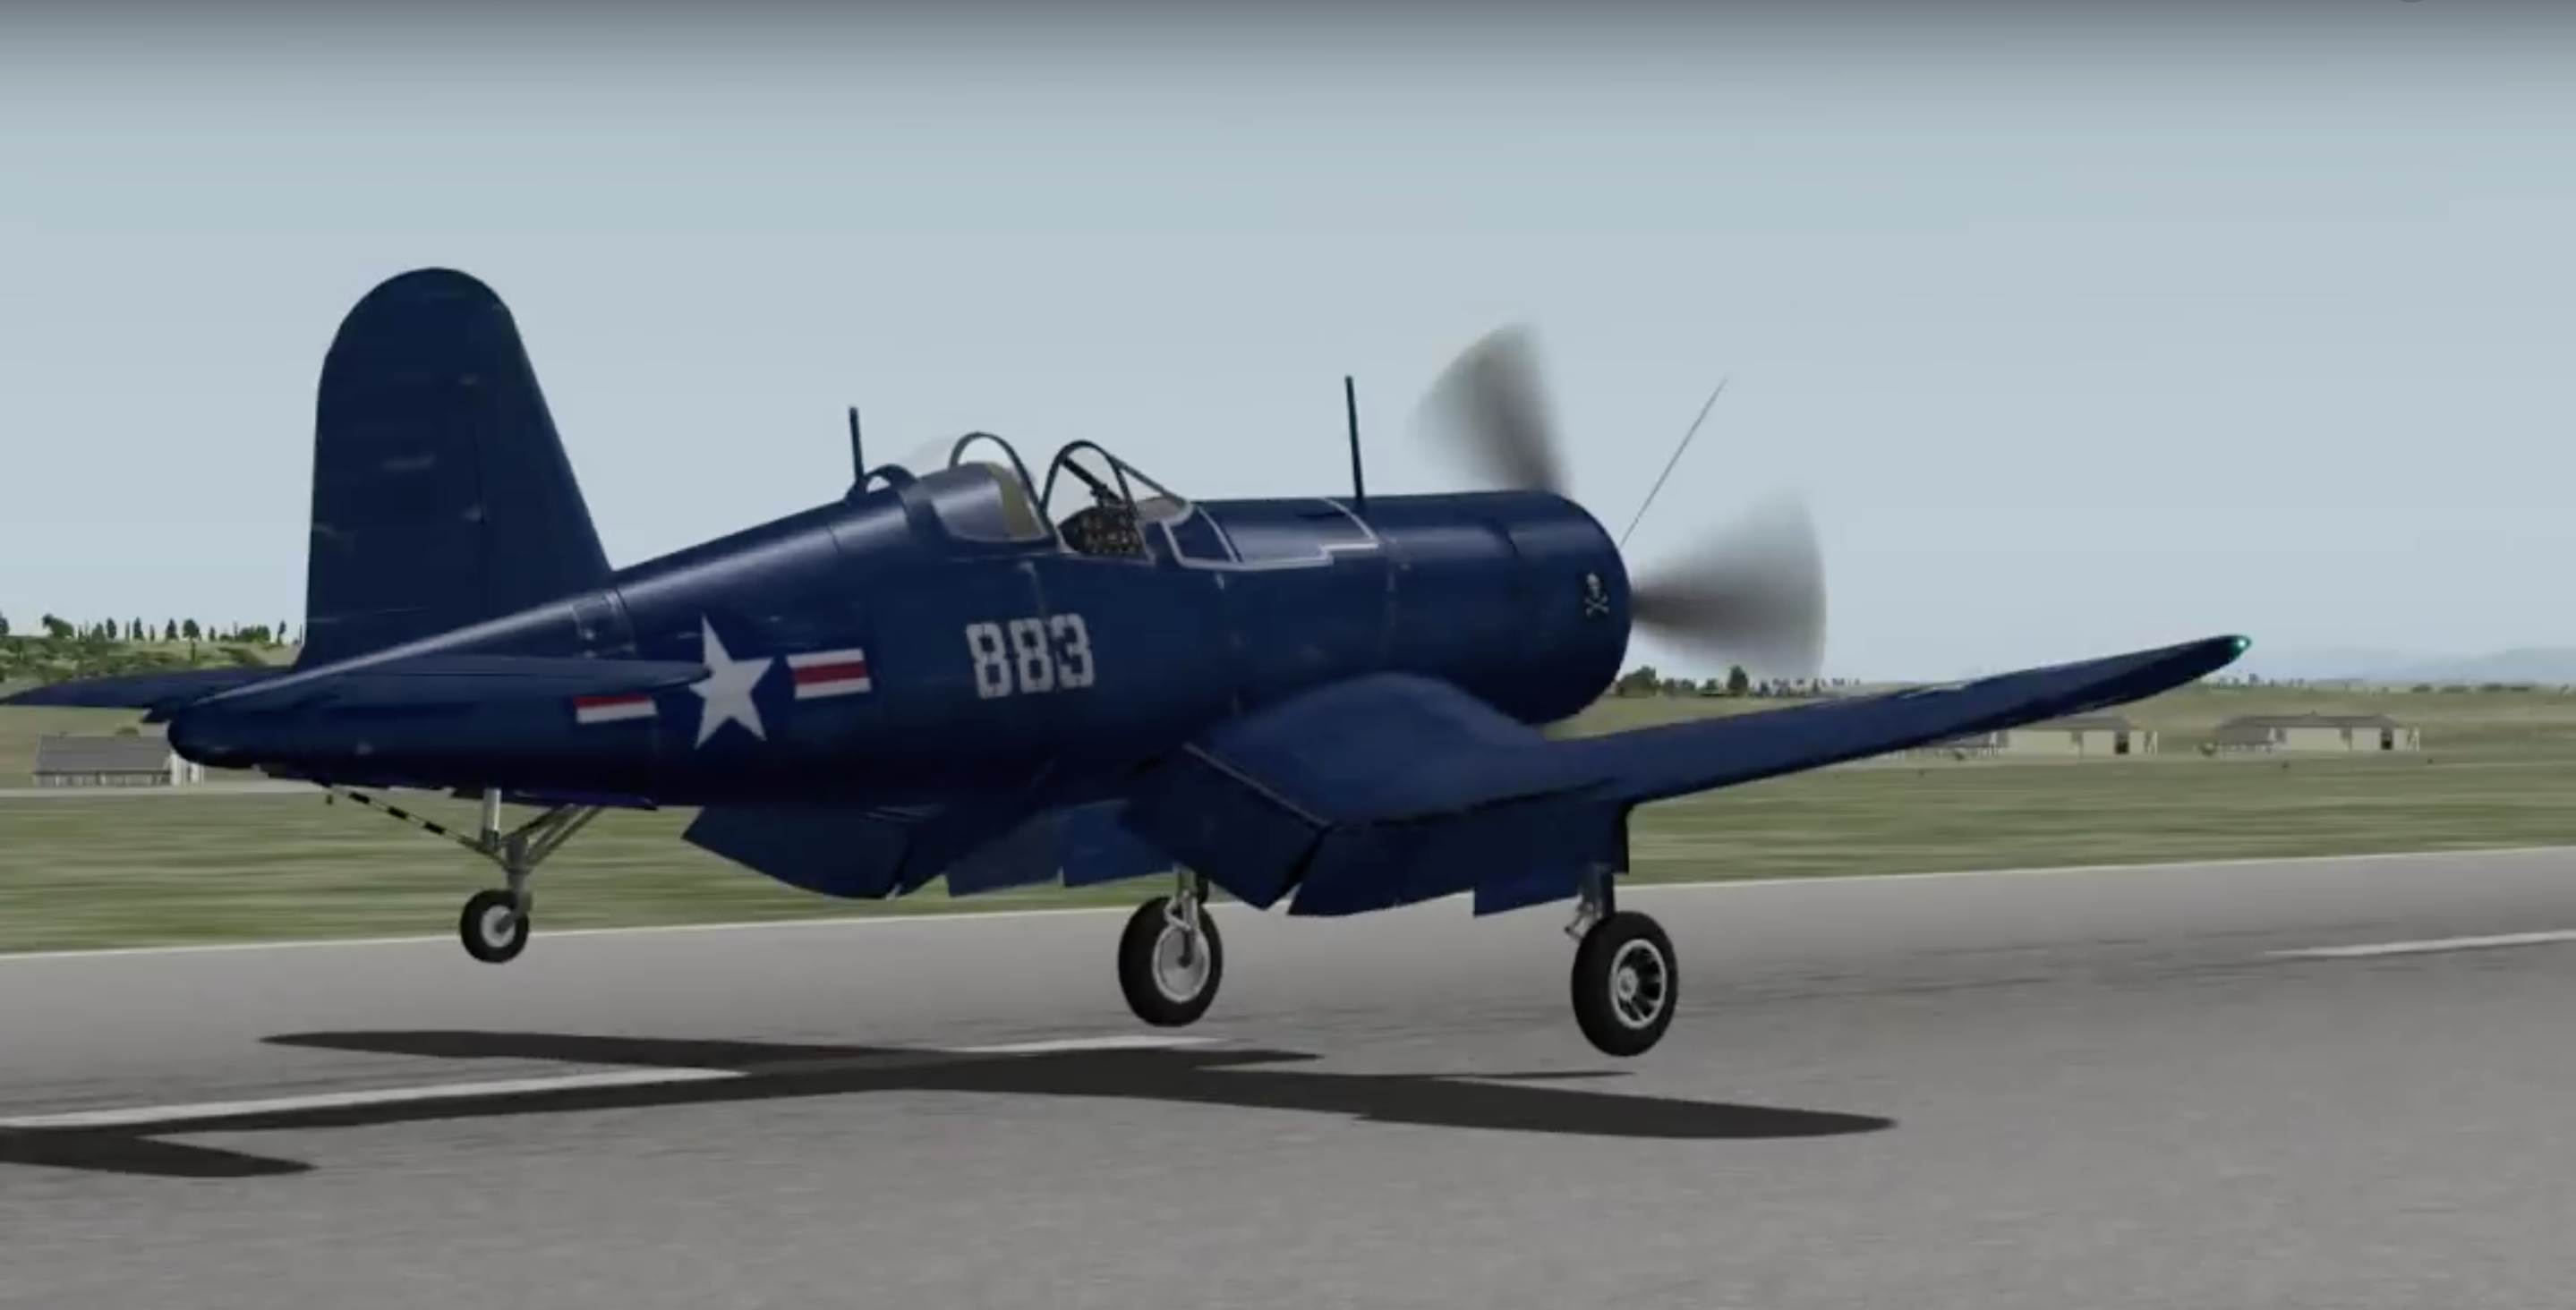
\includegraphics[width=0.85\textwidth]{corsair.png}
  \caption{F4U Corsair model - X-Plane10}
  \label{fig:corsair}
\end{figure}

The \Lone adaptive controller significantly reduces the attitude excursion due to flaps and landing gear.
\begin{figure}[h!]
 \centering
  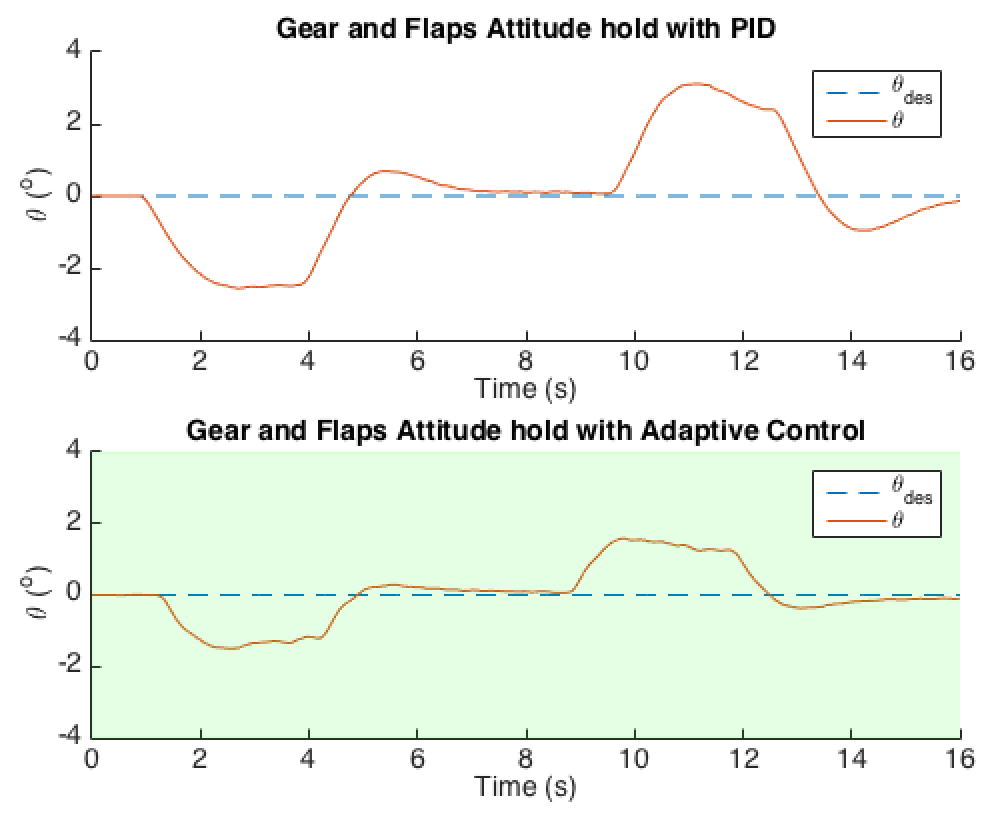
\includegraphics[width=0.85\textwidth]{gear_and_flaps.png}
  \caption{Pitch Attittude Response due to Gear and Flaps}
  \label{fig:gear_and_flaps}
\end{figure}

%---------------------------------------------
\subsection{Roll Performance}
Adaptive control offered little improvement to roll performance with respect to the nominal attitude retention.  The roll axis for multiple aircraft was typically seen to have higher cutoff frequencies with respect to pitch and therefore required higher values for the $D(s)$ cut off frequencies.
\begin{figure}[h!]
 \centering
  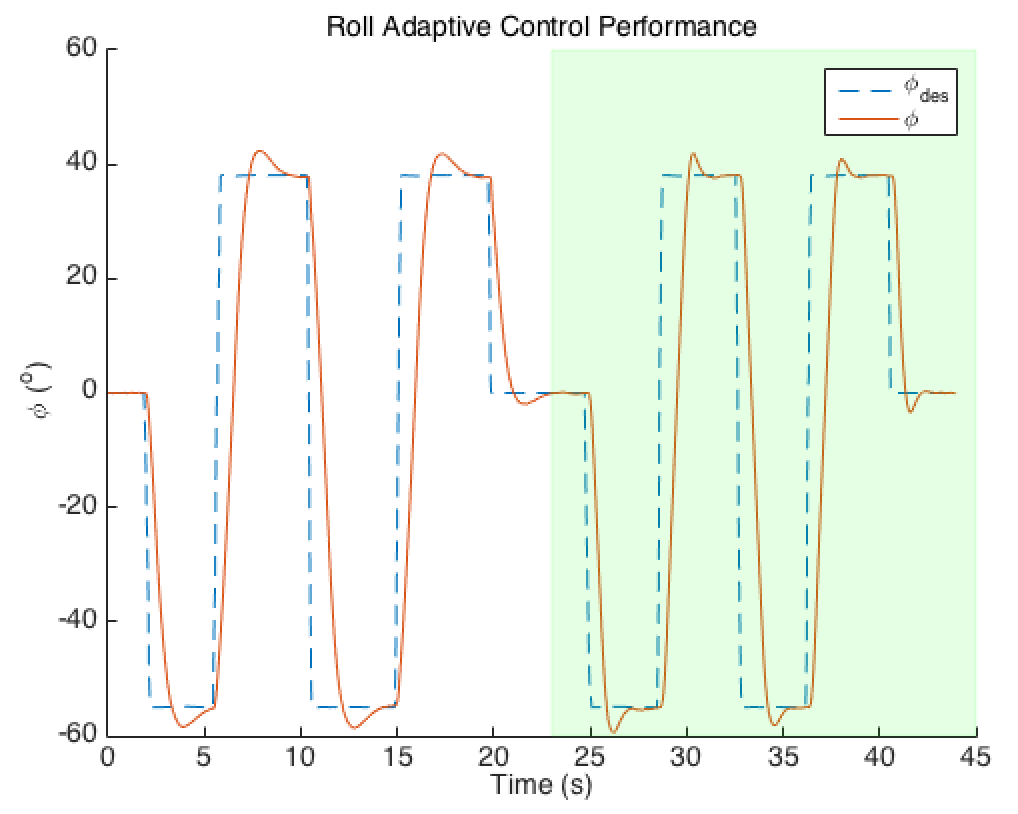
\includegraphics[width=0.85\textwidth]{roll_perf.png}
  \caption{Roll Attittude Performance}
  \label{fig:roll_perf}
\end{figure}

\subsection{Yaw to Roll Coupling}
The roll dynamics are coupled to the yaw dynamics as seen in equation~\ref{eq:aero_torques}.  In the case of an actuator/servo hardover in the yaw channel, the coupling causes unwanted rolling moments.  Figure~\ref{fig:rudder_failure} compares a left and right yaw servo hard over for both \ac{PID} and the \Lone controller.
\begin{figure}[h!]
 \centering
  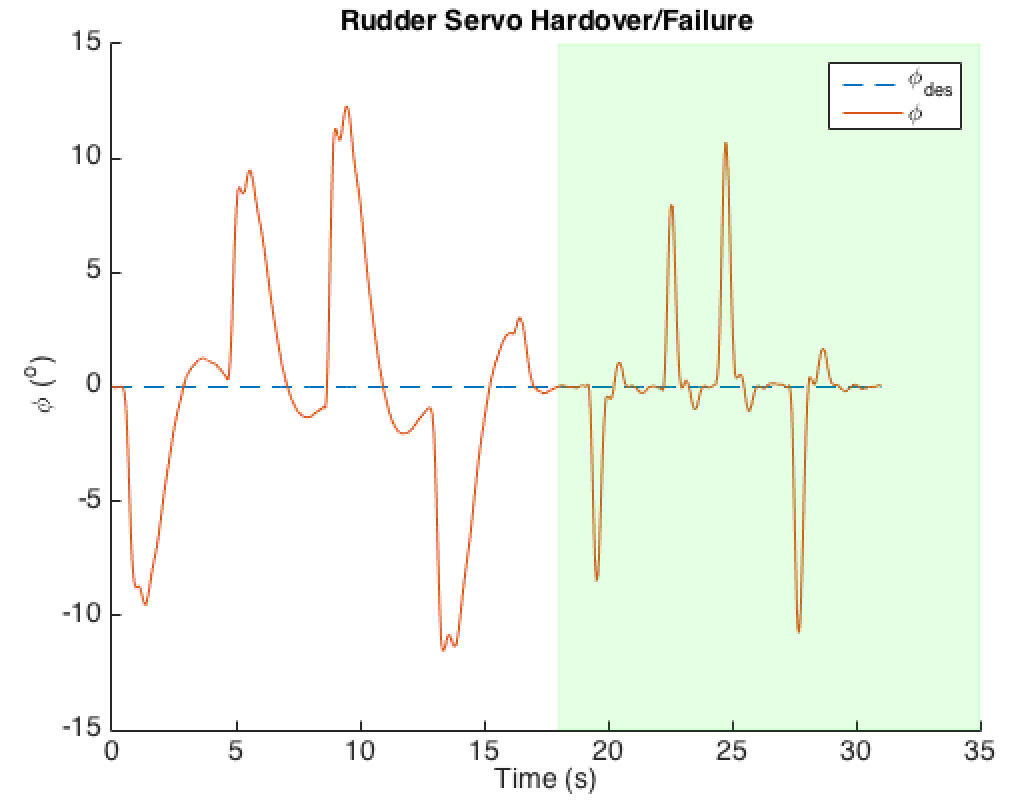
\includegraphics[width=0.85\textwidth]{rudder_failure.png}
  \caption{Roll Response to Rudder Servo Hardover/Failure}
  \label{fig:rudder_failure}
\end{figure}
The adaptive controller significantly outperforms the \ac{PID} controller in maintaining the desired roll.  It could be argued that the \ac{PID} controller's integrator time constant could be re-tuned to be comparable.  It was evident for each of the simulation tests that tuning the \ac{PID} for every scenario would likely have been possible individually to achieve similar performance to the \Lone.  However, the \Lone was not tuned between each of these tests and outperformed \ac{PID} in most, if not all cases.

\subsection{Actuator Miscalibration}
The \Lone adaptive control provided fast learning of airframe actuator miscalibrations.  The autopilot parameter SERVOX\_TRIM was used to offset the ailerons by 15\% of their travel to evaluate how quickly the controller was capable of adapting to the new offset.  This was tested first on the \ac{PID} controller and then on the \Lone as seen in figure~\ref{fig:trim_learn}.
\begin{figure}[h!]
 \centering
  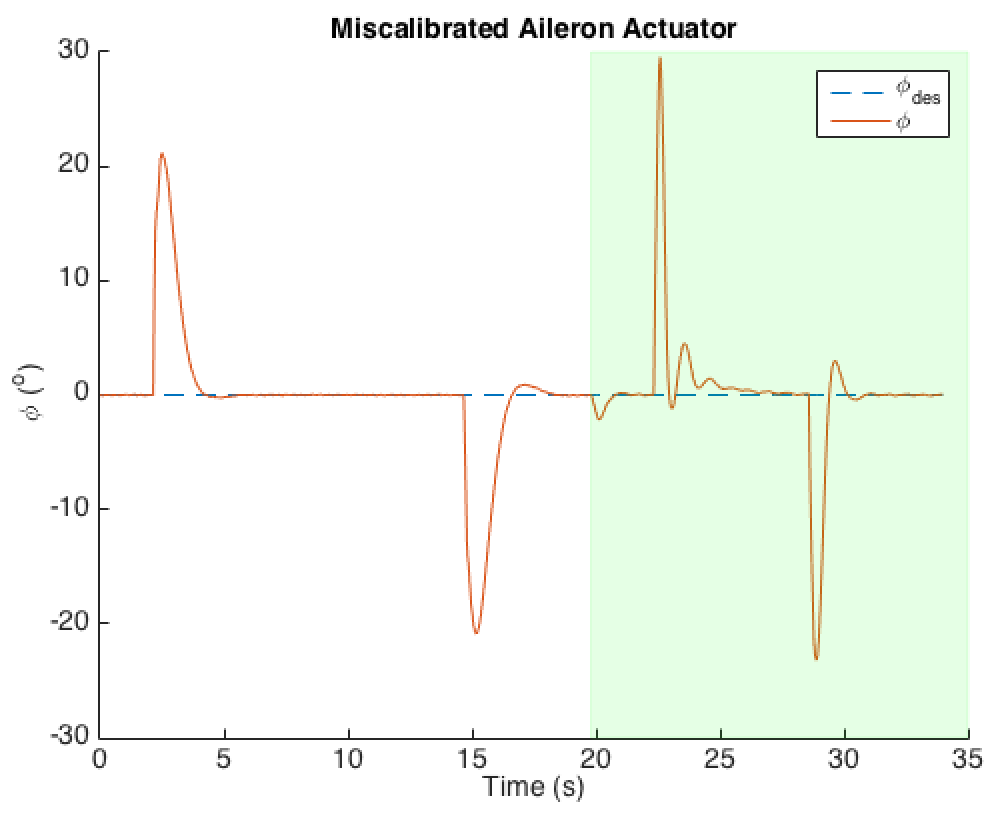
\includegraphics[width=0.85\textwidth]{trim_learn.png}
  \caption{Roll Response to Miscalibrated Aileron Servo}
  \label{fig:trim_learn}
\end{figure}
\begin{figure}[h!]
 \centering
  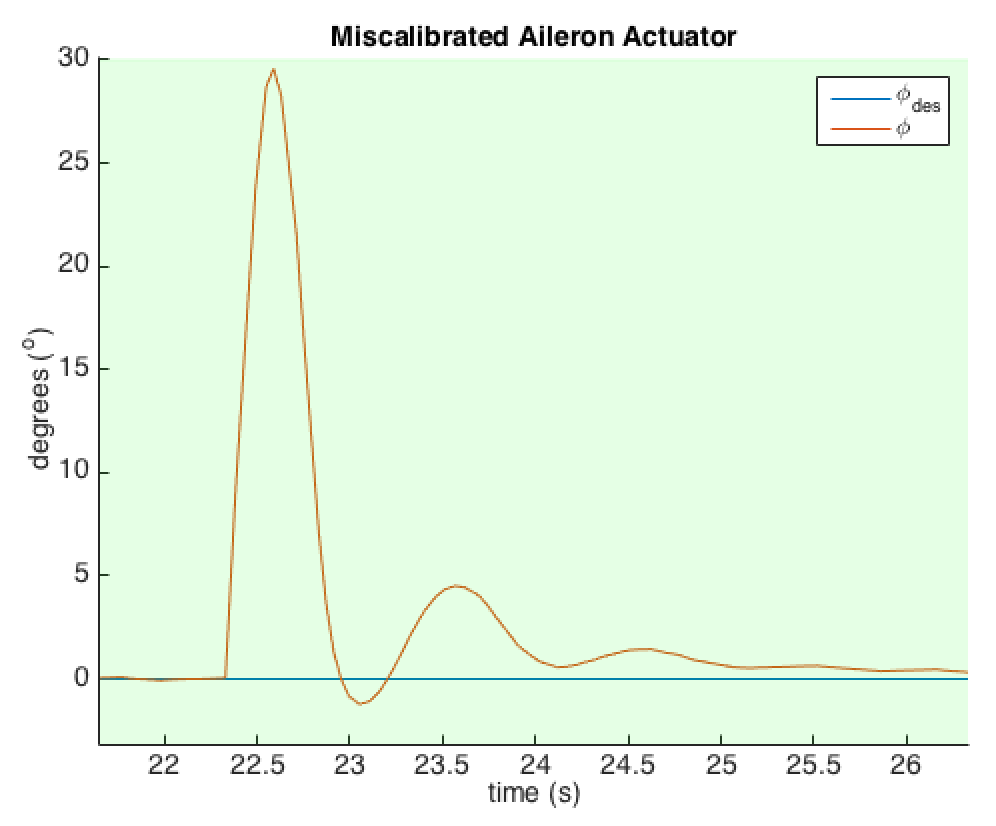
\includegraphics[width=0.65\textwidth]{trim_learn2.png}
  \caption{\Lone Fast Adaptation to Unknown Miscalibration}
  \label{fig:trim_learn2}
\end{figure}

It can be seen in figure~\ref{fig:trim_learn} and \ref{fig:trim_learn2} that the new trim value achieves the reference command in about 0.5 seconds for the \Lone.  The \Lone is slightly faster than \ac{PID}, but the \Lone exhibits some overshoot.  It is important to note that this rate of learning is perfectly adequate for learning the miscalibrations in flight, but is insufficient for learning on take off.  In the takeoff circumstance, the algorithm saturates the actuator if biases exist between desired and achieved.  Because the aircraft has no dynamic pressure, the desired cannot be achieved.  This causes controller saturation, which cannot be unwound fast enough for take-off (specifically for tail-dragger configuration).  This has to be handled with ad-hoc heuristics very delicately.  One could choose to speed scale the learned parameters to help with learning rate, but it was not chosen for this research because this controller is also utilized in tail-sitter configurations where the zero airspeed would cause the controller to refuse to learn when in \ac{VTOL} mode.

\section{Flight Test Results}\label{sec:flight_test}

\subsection{Data Collection}
The Pixhawk autopilot was used to capture roll and pitch rates $(\dot{p},\dot{q})$ for the test vehicle as well as the pilot's command inputs.  These outputs and inputs were the essential building blocks for creating pitch rate and roll rate models for the test vehicle.  The autopilot is capable of logging data at 50-400 Hz and therefore is a discrete time domain signal.  This data should ultimately be manipulated into the s-domain.  The mathematics for this procedure are well defined, and numerous tools can be used to simplify this process.  

It is crucial to ensure there is sufficient frequency content in the data recorded.  Exciting multiple frequencies in the time domain ensures the regression techniques have an adequate sample space to search for polynomial coefficients.  Exciting adequate frequency inputs is analogous to only sampling at one independent variable and expecting to get a regression fit from a non-changing dependent variable.  

To ensure sufficient frequency content was obtained from the aircraft, a linear chirp was chosen and implemented into the Pixhawk source code as follows:

\begin{equation}
x(t)=sin\left[\phi_0+2\pi\left(f_0t+\frac{k}{2}t^2\right)\right]
\end{equation}

where:
\begin{itemize}
 \item[] $\phi_0$ is the initial phase of the chirp at t=0 (nominally zero degrees)
 \item[] $f_0$ is the initial frequency at t=0
 \item[] $k$ is the chirp rate
 \item[] $t$  is time in seconds
\end{itemize}

An example of this formulation can be seen below:

\begin{figure}[!h]
 \centering
  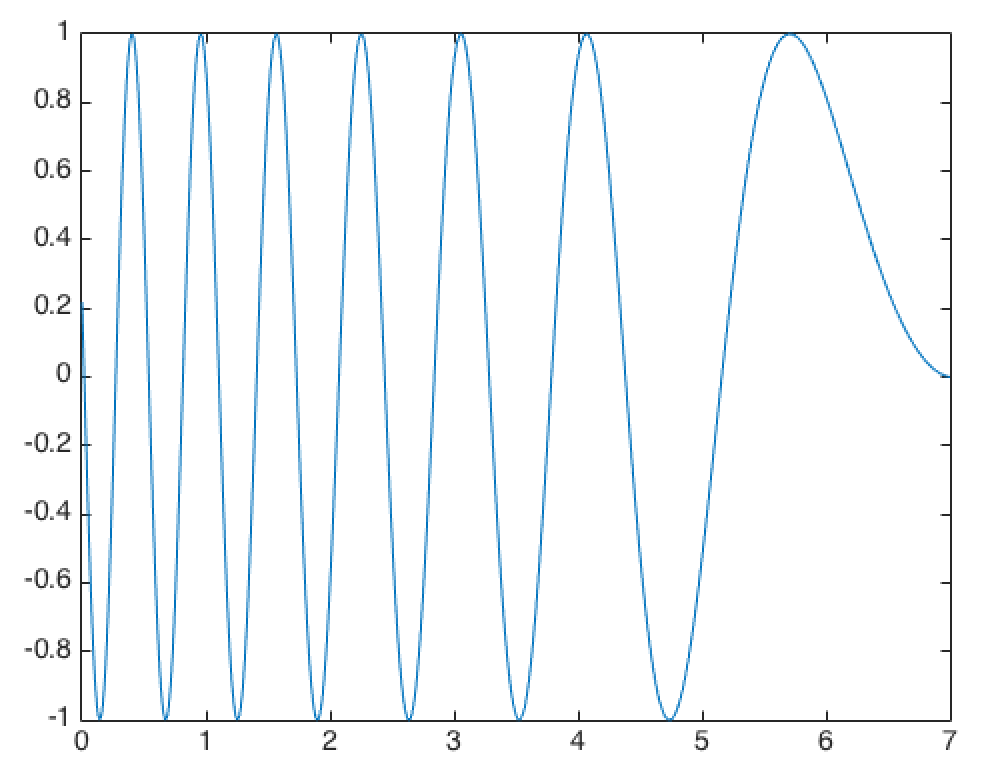
\includegraphics[width=0.50\textwidth]{chirp.png}
  \caption{Reverse Linear Chirp Example}
  \label{fig:chirp}
\end{figure}




